\setcounter{chapter}{0}	
\chapter{مقدمه}

\section{ خونریزی درون‌جمجمه‌ای و اهمیت آن}

خونریزی‌ درون‌جمجمه‌ای
\LTRfootnote{Intracranial Hemorrhage}
یک وضعیت اضطراری پزشکی است که تشخیص سریع و دقیق آن به‌منظور درمان مؤثر بیمار و کاهش خطر ناتوانی شدید یا مرگ، حیاتی است \cite{grewal2018radnet}.
خونریزی درون جمجمه‌ای
می‌تواند به دلایل مختلفی از جمله آسیب مغزی تروماتیک
\LTRfootnote{Traumatic Brain Injury}
، بیماری‌های عروقی، یا مشکلات مادرزادی ایجاد شود و بر اساس محل خونریزی در مغز طبقه‌بندی می‌شود \cite{monica2022detection}.
 به‌صورت تقریبی سالانه بین 40000 تا 67000 بیمار دارای
خونریزی درون جمجمه‌ای
   در ایالات متحده آمریکا شناسایی می‌شوند که نرخ مرگ‌ومیر آنها در 30 روز اول حادثه در حدود 40 درصد است که در نتیجه آن، 
خونریزی درون جمجمه‌ای
   به یکی از بیماری‌ها با بیشترین آمار مرگ‌ومیر تبدیل شده است. این در حالی است که عوارض دیگر این بیماری نیز بسیار خطرناک است، به‌عنوان‌مثال بیشتر از 46 درصد بیماران که دارای نوع خاصی از خونریزی درون‌جمجمه‌ای هستند، پس از بهبود به‌صورت دائمی دچار اختلالات شناختی می‌شوند
 \cite{arbabshirani2018advanced,burduja2020accurate,morgenstern2010guidelines,van2010incidence,hackett2000health}.

  باتوجه‌به نرخ بالای مرگ‌ومیر مرتبط با 
  خونریزی درون جمجمه‌ای
  ، تشخیص سریع و دقیق 
  خونریزی درون جمجمه‌ای
  با استفاده از روش‌های تصویربرداری ضروری است \cite{kuo2019expert}. سی‌تی‌اسکن
 \LTRfootnote{Computed Tomography Scan}
   شایع‌ترین روش برای تشخیص سریع خونریزی به‌ویژه در مراکز فوریت‌های پزشکی به‌حساب می‌آید که دقت مناسب را برای تشخیص این بیماری به متخصصین می‌دهد \cite{ye2019precise,grewal2018radnet,arbabshirani2018advanced,chilamkurthy2018deep}.


\section{انواع خونریزی درون‌جمجمه‌ای}
با پاره شدن عروق شریانی مغز، خون از درون عروق اصلی وارد بافت مغز می‌شود؛ این مسئله در حالی است که لخته‌شدن خون در داخل بدن سخت‌‌تر انجام می‌شود و به‌موجب آن خون وارد بافت مغز شده و با افزایش فشار داخل جمجمه، به بافت‌های حیاتی صدمات جدی وارد می‌کند.  
همان‌طور که در
  \autoref{fig:ch1-brain-ich}
  مشخص است، با پاره شدن شریان‌های خونی درون مغز، خونی که وارد بافت مغز شده است و یک ضایعه بزرگ خونریزی را ایجاد کرده و این ضایعه در تصویر سی‌تی‌اسکن به‌صورت یک بافت که رنگ روشن‌تری نسبت به محیط اطراف دارد قابل‌شناسایی است.
   ‎
\begin{figure}[H]
\centering
\includegraphics[width=1.0\linewidth]{"Images/Chapter1/brain - ich"}
\caption{خونریزی درون‌جمجمه‌ای
\cite{healthjade_intracerebral_hemorrhage}}
\label{fig:ch1-brain-ich}
\end{figure}
خونریزی درون جمجمه‌ای متناسب با محل وقوع به زیرگروه‌های مختلفی تقسیم می‌شوند؛
این طبقه‌بندی شامل خونریزی اپیدورال
\lr{(EDH)}\LTRfootnote{Epidural}
 ، خونریزی ساب‌دورال
 \lr{(SDH)}\LTRfootnote{Subdural}
  ، خونریزی ساب‌آراکنوئید
 \lr{(SAH)}\LTRfootnote{Subarachnoid}
   ، خونریزی پارانشیم مغزی 
 \lr{(CPH)}\LTRfootnote{Cerebral Parenchymal}
   ، و خونریزی داخل بطنی
 \lr{(IVH)}\LTRfootnote{Intraventricular }
  است \cite{burduja2020accurate,hssayeni2020intracranial}.
  در
 \autoref{table: subtype}
 نمونه‌هایی از زیرگروه‌های خونریزی درون‌جمجمه‌ای، محل خونریزی، زمینه، علت وقوع، شکل و علائم بالینی نشان‌داده‌شده است؛ همان‌طور که از تصاویر مشخص است، تشخیص بعضی از انواع خونریزی ‌درون‌جمجمه‌ای به علت حضور در اطراف بقیه بافت‌های مغز،‌ خصوصا جمجمه که از تراکم بیشتری برخوردار است و یا شکل پیچیده‌ای که دارند، حتی برای متخصصین نیز دشوار است.
  
  
\begin{table}[ht]
\centering
\adjustbox{max width=\textwidth,max totalheight=\textheight,keepaspectratio}{
\begin{tabular}{|c|p{7cm}|p{7cm}|p{7cm}|p{7cm}|p{7cm}|}
\hline
\textbf{} & \textbf{\lr{CPH}} & \textbf{\lr{IVH}} & \textbf{\lr{SAH}} & \textbf{\lr{SDH}} & \textbf{\lr{EDH}} \\ \hline
\textbf{محل} & داخل مغز & داخل بطن & بین عنکبوتیه و نرم‌شامه & بین سخت‌شامه و عنکبوتیه & بین سخت‌شامه و جمجمه \\ \hline
\textbf{تصویر} & 
\parbox[c][7cm][c]{7cm}{\centering 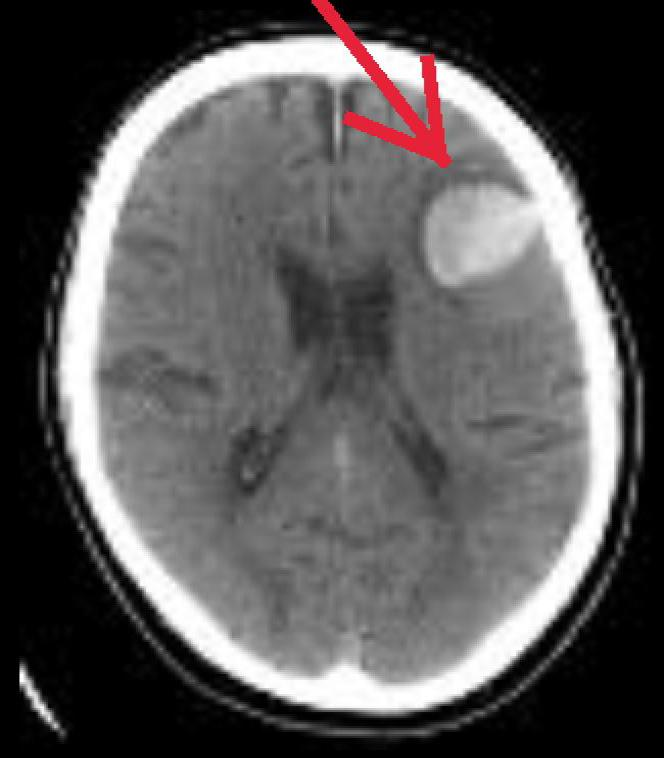
\includegraphics[width=6cm]{"Images/Chapter1/intraparenchymal.JPG"}} & 
\parbox[c][7cm][c]{7cm}{\centering 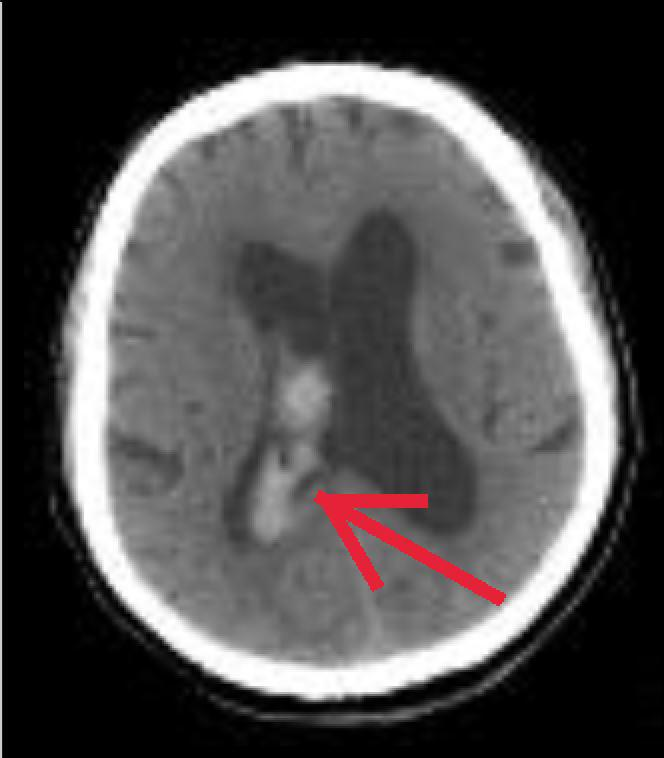
\includegraphics[width=6cm]{Images/Chapter1/intraventricular.JPG}} & 
\parbox[c][7cm][c]{7cm}{\centering 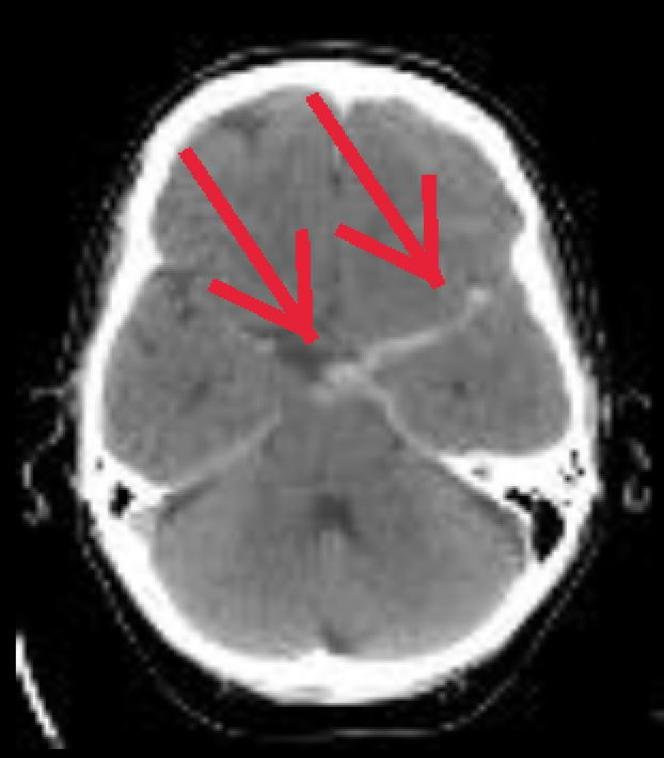
\includegraphics[width=6cm]{Images/Chapter1/subarachnoid.JPG}} & 
\parbox[c][7cm][c]{7cm}{\centering 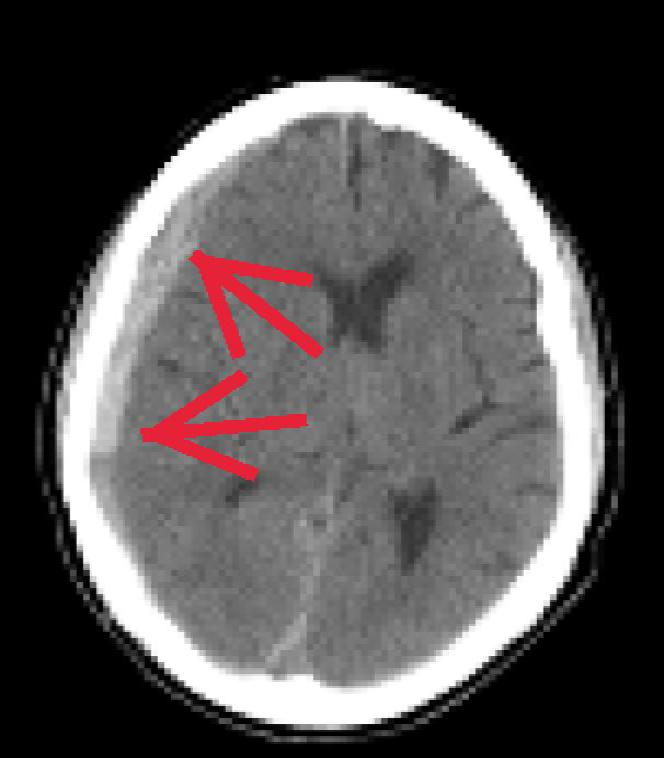
\includegraphics[width=6cm]{Images/Chapter1/subdural.JPG}} & 
\parbox[c][7cm][c]{7cm}{\centering 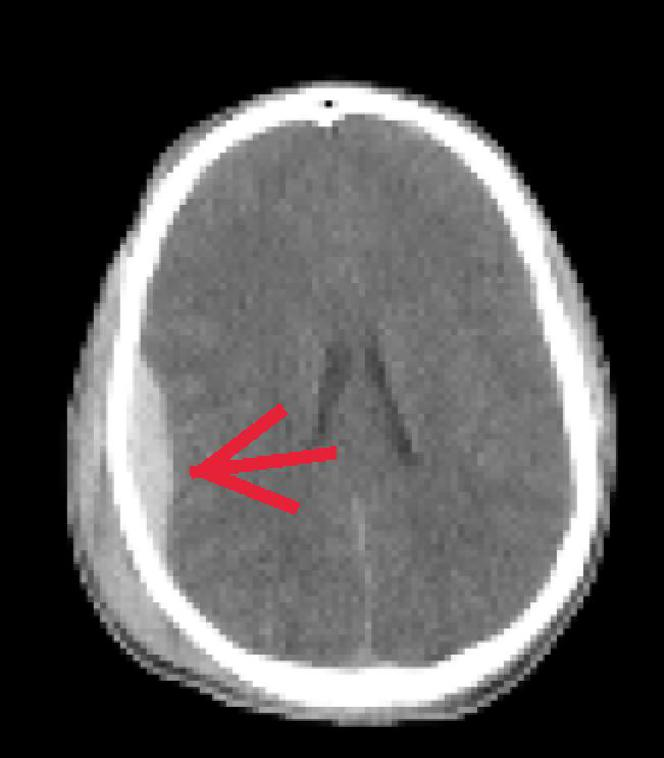
\includegraphics[width=6cm]{Images/Chapter1/Epidural.JPG}} \\ \hline
\textbf{زمینه‌ها} & فشار خون بالا، ضربه، ناهنجاری‌های شریانی-وریدی، تومور، و غیره & می‌تواند با خونریزی‌های درون‌مغزی و زیرعنکبوتیه همراه باشد & پارگی آنوریسم یا ناهنجاری‌های شریانی-وریدی یا ضربه & ضربه & ضربه یا پس از جراحی \\ \hline
\textbf{علت وقوع} & شریانی یا وریدی & شریانی یا وریدی & عمدتاً شریانی & وریدی (وریدهای پل‌زن) & شریانی \\ \hline
\textbf{شکل} & معمولاً گرد & مطابق با شکل بطن & در امتداد شیارها و شکاف‌ها & هلالی & عدسی‌شکل \\ \hline
\textbf{علائم بالینی} & حاد (شروع ناگهانی سردرد، حالت تهوع، استفراغ) & حاد (شروع ناگهانی سردرد، حالت تهوع، استفراغ) & حاد (بدترین سردرد زندگی) & ممکن است تدریجی باشد (بدتر شدن سردرد) & حاد (شکستگی جمجمه و تغییر وضعیت ذهنی) \\ \hline
\end{tabular}}
\caption{انواع زیرگروه‌های خونریزی درون‌جمجمه‌ای
\cite{rsna_hemorrhage_detection_kaggle}}
\label{table: subtype}
\end{table}

  
\section{روش‌های مرسوم در تشخیص خونریزی درون‌جمجمه‌ای}

در حال حاضر تصاویر سی‌تی‌اسکن، به‌عنوان استاندارد اصلی و غیرتهاجمی
\LTRfootnote{Non-invasive}
برای تشخیص خونریزی‌ درون‌جمجمه‌ای است. سی‌تی‌اسکن یک نوع تصویر پرتونگاری
\LTRfootnote{Radiography}
سه‌بعدی است که متشکل از تصاویر دوبعدی از اندام بدن است. روش عمومی پردازش تصاویر سی‌تی‌اسکن به‌صورت دستی انجام می‌پذیرد که به‌موجب آن متخصصین پرتونگاری
\LTRfootnote{Radiology}
 و پزشکی، با بررسی برش‌های
\LTRfootnote{ُSlice}
سی‌تی‌اسکن را به‌صورت مجزا بررسی می‌کنند و مناطق خونریزی را تشخیص می‌دهند. این فرایند به دلیل وابستگی به تخصص و تجربه فردی، شرایط محیطی و فشار کاری، زمان‌بر و مستعد خطا است. \cite{arbabshirani2018advanced,grewal2018radnet,ye2019precise,chilamkurthy2018deep,kuo2019expert}.
فرایند بررسی دستی تصاویر سی‌تی‌اسکن، زمان‌بر بوده و به‌شدت به دردسترس‌بودن پرتونگار‌های 
\LTRfootnote{Radiologist}
باتجربه بستگی دارد \cite{burduja2020accurate}.
 در شرایط اضطراری، خصوصا در مراکز فوریت‌های پزشکی، زمانی که برای پردازش برش‌های سی‌تی‌اسکن صرف می‌شود، می‌تواند به طور قابل‌توجهی در نتایج درمان بیمارها تأثیر بگذارد؛ این مسئله در مواردی از اهمیت بیشتری برخوردار می‌شود که درمان بیمار نیازمند مداخله فوری گروه پزشکی است \cite{chilamkurthy2018deep}. نکته حائز اهمیت در روش معمول برای بررسی تصاویر سی‌تی‌اسکن در مراکز پزشکی این است که بررسی اولیه تصاویر، توسط پزشکان و پرتونگار‌هایی باتجربه کمتر انجام می‌شود و در مراحل بعدی این تصاویر توسط متخصصینی باتجربه بیشتر بررسی می‌شود. تعدادی از مطالعات نشان داده‌اند که در روش مذکور،‌ بین پزشکان و پرتونگار‌هایی که در مرحله اول تصاویر را بررسی می‌کنند و پزشکان و پرتونگار‌هایی که در ادامه این تصاویر را بررسی می‌کنند،‌ اختلاف‌نظر وجود دارد که این مسئله می‌تواند منجر به عواقب جبران‌ناپذیر گردد
\cite{ye2019precise, alfaro1995accuracy, lal2000clinical, erly2002radiology, strub2007overnight}.
   احتمال خطای انسانی در بررسی دستی تصاویر پیچیده و سه‌بعدی سی‌تی‌اسکن، از دیگر نقاط ضعف روش معمول پردازش این تصاویر است، به‌ویژه در محیط‌های شلوغ و پرتنش که پرتونگار‌ها ممکن است تحت فشار زیاد باشند \cite{ye2019precise}.
   
\section{روش‌های رایانه‌ای در پردازش تصاویر پزشکی}
اهمیت مسئله خونریزی درون‌جمجمه‌ای و چالش‌های مرتبط با آن در بخش قبل مورد بررسی قرار گرفت، روش‌های مبتنی‌ بر پردازش رایانه‌ای
\LTRfootnote{Computer}
تصاویر پزشکی، می‌تواند یک راه‌حل مناسب برای رفع نقاط ضعف روش کنونی بررسی تصاویر پزشکی باشد
\cite{grewal2018radnet, arbabshirani2018advanced, ye2019precise, lee2019explainable, chang2018hybrid, chilamkurthy2018deep, titano2018automated, kuo2019expert}.
 ابزارهای خودکار برای تشخیص و کمیت‌سنجی خونریزی، از پیشرفت‌های روش‌های یادگیری ماشین 
\LTRfootnote{Machine Learning}
و یادگیری عمیق
\LTRfootnote{Deep Learning}
 و سامانه‌های
 \LTRfootnote{System}
  تشخیص به کمک رایانه 
 \LTRfootnote{Computer-aided Diagnosis}
 استفاده می‌کنند تا تجزیه‌وتحلیل سریع و دقیقی از تصاویر سی‌تی‌اسکن ارائه دهند. با خودکارسازی تشخیص خونریزی درون‌جمجمه‌ای و استفاده از آنها به‌صورت نظر ثانویه
  \LTRfootnote{ُSecond Opinion}
 ، این سامانه‌ها می‌توانند بار کاری پرتونگار‌ها را کاهش دهند، دقت تشخیص را افزایش دهند از اشتباهات متخصصین جلوگیری کنند، زمان تشخیص را به حداقل برسانند، بعضی از هزینه‌های فرایند درمان را به علت کاهش دخالت انسانی کاهش دهند و به‌صورت کلی فرایند تشخیص را بهبود ببخشند که این موارد به بهبود نتایج بیماران منجر خواهد شد. بااین‌حال، ضمن اینکه سامانه‌های تشخیص به کمک رایانه نویدبخش هستند؛ اما امکان خطا در آنها وجود دارد که می‌تواند تصمیم‌گیری بالینی را با مشکلاتی روبرو کند؛ بنابراین، ادغام این ابزارها در عمل باید با دقت انجام شود \cite{titano2018automated}.
 
 
 
 \section{مجموعه‌داده‌ها}
 
 
 در سال‌های اخیر، مجموعه‌داده‌های متعددی برای پشتیبانی از توسعه مدل‌های
 \LTRfootnote{Model}
  یادگیری عمیق در حوزه تصویربرداری پزشکی، به‌ویژه برای طبقه‌بندی خونریزی درون‌جمجمه‌ای ایجاد شده‌اند. در ادامه به بررسی برخی از مهم‌ترین مجموعه‌داده‌هایی که در این حوزه مورد استفاده قرار گرفته‌اند، می‌پردازیم.
 
 \subsection{مجموعه‌داده‌ی انجمن پرتوشناسی آمریکای شمالی
  \lr{(RSNA)}}
 مجموعه‌داده‌ی 
 \lr{RSNA Intracranial Hemorrhage Detection}\cite{rsna_hemorrhage_detection_kaggle,rsna_kaggle}
  که برای چالش یادگیری ماشین سال ۲۰۱۹ انجمن پرتونگاری آمریکای شمالی جمع‌آوری شده است، یکی از منابع برجسته در زمینه طبقه‌بندی خونریزی درون‌جمجمه‌ای محسوب می‌شود. این مجموعه‌داده،از چند مرکز پرتونگاری جمع‌آوری شده است که سه مؤسسه دانشگاه استنفورد در ایالات متحده، دانشگاه فدرال سائوپائولو در برزیل و بیمارستان دانشگاه توماس جفرسون در ایالات متحده شامل آنها می‌باشد. این مجموعه شامل تصویر سی‌تی‌اسکن مغزی ۲۵۳۱۲ بیمار است که از این میان، ۸۸۸۹ بیمار دارای انواع مختلف خونریزی درون‌جمجمه‌ای هستند. تصاویر سی‌تی‌اسکن درون این مجموعه‌داده در سطح برش،‌ حاشیه‌نویسی 
   \LTRfootnote{Annotation}
 شده‌اند.  تصاویر سی‌تی‌اسکن در این مجموعه‌داده به‌صورت فایل‌های
  \lr{DICOM}
  \LTRfootnote{Digital Imaging and Communications in Medicine}
   ارائه شده‌اند که استانداردی برای تصویربرداری پزشکی است. این مجموعه‌داده به طور گسترده‌ای در طبقه‌بندی انواع خونریزی مورد استفاده قرار گرفته و به‌عنوان منبعی بنیادی برای آموزش و اعتبارسنجی مدل‌های یادگیری ماشین که به طبقه‌بندی خونریزی درون‌جمجمه‌ای تبدیل شده است.
 
 \subsection{مجموعه‌داده‌ی \lr{MosMed}}
 مجموعه‌داده‌ی
  \lr{MosMed}\cite{medmos_khoruzhaya2024expanded}،
  یک مجموعه‌داده خونریزی درون‌جمجمه‌ای است که در روسیه جمع‌آوری شده است. این مجموعه‌داده به طور خاص برای تسهیل توسعه ابزار‌های هوش مصنوعی به‌منظور تشخیص و طبقه‌بندی خونریزی درون‌جمجمه‌ای طراحی شده است. این مجموعه شامل سی‌تی‌اسکن مغزی ۸۰۰ بیمار است که 400 بیمار دارای خونریزی درون‌جمجمه‌ای هستند. این مجموعه‌داده درسطح بیمار حاشیه‌نویسی شده است و تصاویر آن به‌صورت فایل‌های 
  \lr{DICOM}
  دردسترس قرار دارد.
 
 \subsection{مجموعه‌داده‌ی \lr{CQ500}}
 مجموعه‌داده‌ی
  \lr{CQ500}\cite{cq500_chilamkurthy2018development}
  ، یک مجموعه‌داده مهم است که از چند مرکز متفاوت شامل پنج مرکز مختلف در هند است. این مجموعه‌داده حاوی ۴۹۱ سی‌تی‌اسکن سر است که برای انواع خونریزی‌های درون‌جمجمه‌ای در سطح بیمار حاشیه‌نویسی شده‌اند. تصاویر سی‌تی‌اسکن در این مجموعه‌داده به‌صورت فایل
   \lr{DICOM}
    ارائه شده.
 \subsection{مجموعه‌داده‌ی \lr{PHE-SICH-CT-IDS}}
 مجموعه‌داده‌ی 
 \lr{PHE-SICH-CT-IDS}\cite{PHE_ma2024phe}
 ، اگرچه به‌طور خاص برای خونریزی درون‌جمجمه‌ای جمع‌آوری نشده است، اما به دلیل تمرکز آن بر وظایف طبقه‌بندی، تشخیص و قطعه‌بندی مرتبط به 
 \lr{Perihematomal Edema}
  در خونریزی‌ درون‌جمجمه‌ای قابل‌توجه است. این مجموعه‌داده‌ از بیمارستان 
  \lr{Shengjing}
  در چین جمع‌آوری شده است که 
   شامل تصویر سی‌تی‌اسکن 120 بیمار است که تمامی آنها خونریزی درون‌جمجمه‌ای دارند و حاشیه‌نویسی آنها در سطح برش انجام شده است. تصاویر سی‌تی‌اسکن در این مجموعه‌داده به‌صورت فایل‌های 
   \lr{NIFTI},
   \lr{JPG} و
   \lr{PNG}
   ارائه شده است. مجموعه‌داده‌ی 
   \lr{PHE-SICH-CT-IDS}
    منبعی ارزشمند برای توسعه مدل‌های یادگیری عمیق که هدف آن‌ها طبقه‌بندی، تشخیص یا قطعه‌بندی است. در
   \autoref{fig:ch1-phe-sample}
 چند برش از تصاویر مجموعه‌داده 
 \lr{PHE-SICH-CT-IDS}
 است، همان‌طور  که در این تصویر مشخص است،‌ در اطراف ضایعه خونریزی،‌ یک حاشیه تیره‌تر وجود دارد که به آن 
 \lr{Edma}
 گفته می‌شود و این ضایعه قطعه‌بندی شده است؛ همچنین این مجموعه‌داده حاشیه‌نویسی مناسب برای وظیفه تشخیص را نیز دارد.
 \begin{figure}[H]
 \centering
 \includegraphics[width=1.0\linewidth]{"Images/Chapter1/PHE sample"}
 \caption{چند نمونه تصویر از مجموعه‌داده 
 \lr{PHE-SICH-CT-IDS}}
 \label{fig:ch1-phe-sample}
 \end{figure}
 
 \subsection{مجموعه‌داده‌ی \lr{PhysioNet}}
 مجموعه‌داده‌ی خونریزی درون‌جمجمه‌ای 
 \lr{PhysioNet}\cite{physionet_hssayeni2020intracranial}،
 مجموعه‌داده‌ای است که در ادامه این مطالعه از آن استفاده شده است. این مجموعه‌داده
 از بیمارستان
 \lr{Al Hilla}
 در عراق جمع‌آوری شده است و شامل 82 تصویر سی‌تی‌اسکن از بیماران است که 36 نفر از آنها دارای خونریزی درون جمجمه‌ای هستند.
   این مجموعه‌داده، شامل حاشیه‌نویسی‌های مناسب برای وظایف طبقه‌بندی و قطعه‌بندی است که آن را به تنها مجموعه‌داده با دسترسی عمومی تبدیل می‌کند که امکان قطعه‌بندی خونریزی درون‌جمجمه‌ای را فراهم می‌کند. جزئیات  بیشتر درمورد این دیتاست در 
   \autoref{dataset}
 توضیح داده شده است.
 تصویر
 \autoref{fig:ch1-physionet-sample}
 چند نمونه از برش‌های خونریزی درون این مجموعه‌داده را مشخص می‌کند.
 \begin{figure}[H]
 \centering
 \includegraphics[width=1.0\linewidth]{"Images/Chapter1/physionet sample"}
 \caption{چند نمونه تصویر از مجموعه داده
 \lr{PhysioNet}}
 \label{fig:ch1-physionet-sample}
 \end{figure}
 
 
 \section{تحقیقات اخیر در زمینه یادگیری ماشین}
 
 در سال‌های اخیر، یادگیری عمیق پیشرفت‌های قابل‌توجهی در زمینه طبقه‌بندی و قطعه‌بندی خونریزی درون‌جمجمه‌ای داشته است و مطالعات متعددی به بررسی این موضوع پرداخته‌اند. این مدل‌ها نه‌تنها از نظر نوآوری فنی قابل‌توجه هستند، بلکه پتانسیل بالای آنها می‌تواند باعث استفاده از آنها در دستگاه‌های تشخیص و درمان بیمارستان‌ها شود که موجب بهبود عملکرد خدمه درمان، کاهش هزینه‌های درمان، کاهش زمان تشخیص و افزایش دقت در طبقه‌بندی و قطعه‌بندی خونریزی درون‌جمجمه‌ای شود. برخی از این مطالعات، از جمله تحقیقات
  \lr{Titano}\cite{titano2018automated}, \lr{Arbabshirani}\cite{arbabshirani2018advanced} و \lr{Kuo}\cite{kuo2019expert}،
و همکارانشان مدل‌های پیشنهادی خود را در محیط‌های بیمارستانی آزمایش کرده‌اند و نتایج آن‌ها نشان داده است که ابزار‌های هوش مصنوعی می‌توانند به ‌طور مؤثری در بهبود نتایج درمان برای بیماران نقش داشته باشد. به طور خاص، \lr{Titano} و همکاران یک دستگاه خودکار تشخیص خونریزی درون‌جمجمه‌ای مبتنی بر یادگیری عمیق توسعه دادند که این دستگاه توانست 
\lr{Accuracy}
 \(87\%\) و 
 \lr{Sensitivity}
  \(94\%\) کسب کند که عملکرد آن با کارشناسان انسانی قابل مقایسه است، همچنین ابزار هوش مصنوعی پیشنهادی آنها در محیط‌های بالینی به کار گرفته شده است. \lr{Kuo} و همکاران یک شبکه عصبی پیچشی برای طبقه‌بندی خونریزی حاد درون‌جمجمه‌ای با 
  \lr{Accuracy}
   \(99\%\) و \lr{AUC} برابر با
 \(99\%\)
توسعه داده‌اند که نشان‌دهنده قابلیت اطمینان بالا در شرایط بالینی است. سایر مطالعات، مانند
 \lr{Chang}\cite{chang2018hybrid}
  و
   \lr{Chilamkurthy}\cite{chilamkurthy2018deep}
    نیز نتایج قابل‌توجهی در زمینه طبقه‌بندی خونریزی‌ها با استفاده از مدل‌های یادگیری عمیق ارائه کرده‌اند.
 
 \lr{Neethi}\cite{neethi2022stroke} و همکاران 
 مروری بر روش‌های مختلف یادگیری عمیق انجام داده‌اند که از مجموعه‌داده‌های مختلفی از جمله \lr{PhysioNet} و مجموعه‌داده \lr{RSNA} استفاده کردند. آنها از مجموعه‌داده \lr{RSN } که شامل 25312 تصویر سی‌تی‌اسکن از بیماران است، برای آموزش مدل‌های یادگیری عمیق بهره بردند و عملکرد آن را بر روی مجموعه‌داده \lr{PhysioNet} ارزیابی کردند. آن‌ها با استفاده از مدل \lr{ResNet50-V2} بر روی مجموعه‌داده \lr{PhysioNet} به
  \lr{‎Recall}‎ \(76\%\) و \lr{F1 Score}
   برابر با 
   \(67\%\) 
   دست یافتند که این نتایج به‌صورت برش‌محور
   \LTRfootnote{Slice-wise}
   گزارش شده است.
 در میان کارهایی که روی مجموعه‌داده \lr{PhysioNet} انجام شده است،
  \lr{Kyung}\cite{kyung2022improved}
و همکاران
شبکه‌ای به نام 
\lr{SMART-Net} 
را پیشنهاد کردند که به کمک روش انتقال یادگیری
\LTRfootnote{Transfer Learning}
توانسته‌اند به \lr{F1 Score} برابر با
 \(84\%\)
 و 
 \lr{Sensitivity}
 برابر با 
  \(97\%\)
  و 
  \lr{Specificity}
  برابر با
  \(74\%\)
  بیمارمحور 
  \LTRfootnote{Patient-wise}
   دست یابند.
 در ادامه 
 \lr{Hssayeni}\cite{physionet_hssayeni2020intracranial}
 و همکاران، از مدل معروف 
 \lr{U-Net}
 استفاده کرده‌اند تا یک مدل برای قطعه‌بندی تصاویر سی‌تی‌اسکن آموزش دهند. آموزش این مدل با تصاویر ورودی که از ابعاد اصلی برخوردار هستند، باعث شده است تا مدل ماسک‌هایی
 \LTRfootnote{Mask} 
 تماما سیاه تولید کند که به معنی عدم تشخیص هیچ پیکسلی دارای خونریزی می‌باشد. از این نتیجه می‌توان برداشت کرد که معیار 
 \lr{IoU}
 و 
 \lr{Dice}
 در آموزش مدل با ابعاد اصلی برابر 0 بوده است. در ادامه این تحقیق، 
  \lr{Hssayeni}
  و همکاران تصویر ورودی را به قسمت‌های 
  $160\times160$
  تقسیم کرده‌اند که به‌موجب آن هر تصویر سی‌تی‌اسکن، به تعدادی تصویر دارای همپوشانی تبدیل می‌شوند و روی هر پیکسل از تصویر سی‌تی‌اسکن، 4 مرتبه پیش‌بینی انجام می‌شود. آنها با تعدیل تعداد تصاویر دارای خونریزی و تصاویری که خونریزی ندارند به روش‌های کاهش داده غالب
  ‌\LTRfootnote{Undersampling}
   و افزایش مصنوعی داده
   ‌\LTRfootnote{Augmentation}
   و توسعه یک روش شورایی برای تصمیم‌گیری، توانستند معیار شباهت 
   \lr{IoU}
   برابر 
   $21.8\%$
    و معیار 
    \lr{Dice}
    برابر 
    $31.5\%$
    دست پیدا کنند.
    \lr{Li}\cite{li2020deep}
    و همکاران نیز یک مدل 
    \lr{U-Net}
    را روی مجموعه‌داده
    \lr{PhysioNet}
    آموزش داده‌اند؛ اما از جزئیات این آموزش اطلاعات زیادی را مطرح نکرده‌اند. آنها با استفاده از مدل
    \lr{U-Net}
    توانسته‌اند معیار شباهت 
    \lr{IoU}
    برابر 
    $21\%$
    و معیار
    \lr{Dice}
    برابر 
    $35\%$
    را به ‌دست‌ آورده‌اند.
 \subsection{نقاط ضعف موجود در پژوهش‌های گذشته}
 
 
 
 
 با وجود پیشرفت‌های قابل‌توجه در مدل‌های یادگیری عمیق، هنوز چالش‌هایی در تفسیرپذیری مدل‌های شبکه عصبی وجود دارد که می‌توان از آن به‌عنوان یکی از نقاط ضعف ادبیات موجود در این زمینه دانست؛ زیرا تفسیرپذیر بودن ابزار هوش مصنوعی، یکی از معیارهای اساسی برای متخصصین حوزه پزشکی است تا از این ابزار استفاده کنند. از دیگر نقاط ضعف در ادبیات خونریزی درون‌جمجمه‌ای، دردسترس نبودن مجموعه‌داده‌های بزرگ با حاشیه‌نویسی مناسب و مجموعه‌داده‌های مربوط به بیمارستان‌ها و دستگاه‌های موجود در ایران است؛ وجود یک مجموعه‌داده با ابعاد مناسب از دستگاه‌های موجود در ایران، می‌تواند مسیر توسعه یک ابزار هوش مصنوعی در زمینه خونریزی درون‌جمجمه‌ای را در ایران وجود هموار سازد. از دیگر نقاط ضعف موجود در ادبیات موجود در این مسئله، استفاده از شبکه‌هایی با ابعاد بسیار بزرگ توسط محققین است که نیازمند پردازشگر‌هایی با هزینه بیشتر هستند. از مهم‌ترین مشکلات موجود در تحقیقات گذشته، توجه نکرده به بیمارمحور بودن داده‌ها هنگام تفکیک آنها به زیرمجموعه‌های آموزش و ارزیابی اشاره کرد که درنتیجه‌ آن برش‌هایی از یک بیمار که شباهت بسیار زیادی به یکدیگر دارند، در زیرمجموعه‌های آموزش و ارزیابی قرار گیرد که درنتیجه آن همبستگی بین این دو مجموعه‌داده زیاد خواهد شد.
استفاده نکردن از روش مرسوم
\lr{K-Fold-Cross-Validation}، 
یا نداشتن روش شورا در تصمیم‌گیری در این روش، یکی دیگر از معایب موجود در تحقیقات گذشته است که به‌موجب آن، تعمیم‌پذیری مدل به دست آمده از این تحقیقات محل ابهام است.
به‌عنوان یکی از اشکالات مهم در ادبیات موجود، عدم ارائه معیارهای مناسب و کافی برای ارزیابی عملکرد مدل‌های یادگیری ماشین است که در نتیجه آن، نتایج به دست آمده از شفافیت کافی برخوردار نیست.
 \subsection{اهداف پژوهش}
 در این پژوهش تلاش شده تا در گام نخست یک روش دومرحله‌ای شامل یک مدل طبقه‌بندی و یک مدل قطعه‌بندی که به‌صورت متوالی استفاده می‌شوند توسعه داده شود که این روش،  موجب بهبود عملکرد مدل‌های پردازش تصویر در قطعه‌بندی شده است؛ نکته حائز اهمیت در این روش این است که با کاهش امکان ایجاد 
 \lr{False Positive}
 در پیش‌بینی‌های مدل قطعه‌بندی، باعث بهبود عملکرد مدل‌های قطعه‌بندی خواهد شد.
  در گام بعدی یک پس‌پردازش
 \LTRfootnote{Post-process}
  در لایه تصمیم‌گیری توسعه داده شده است که این پس‌پردازش نیز موجب بهبود عملکرد مدل طبقه‌بندی شده است.
 در انتها با استفاده از انواع معیارهای موجود، آموزش مدل با استفاده از روش
 \lr{5-Fold-Cross-Validation}،
  طراحی یک ضابطه تصمیم‌گیری
 \LTRfootnote{Decision Policy}
 
  و استفاده از روش‌هایی برای تفسیر‌پذیر کردن مدل، امکان تحلیل جامع از عملکرد مدل فراهم شده است.
